\documentclass{standalone}
\usepackage{tikz}
\usetikzlibrary{patterns, positioning}


\begin{document}
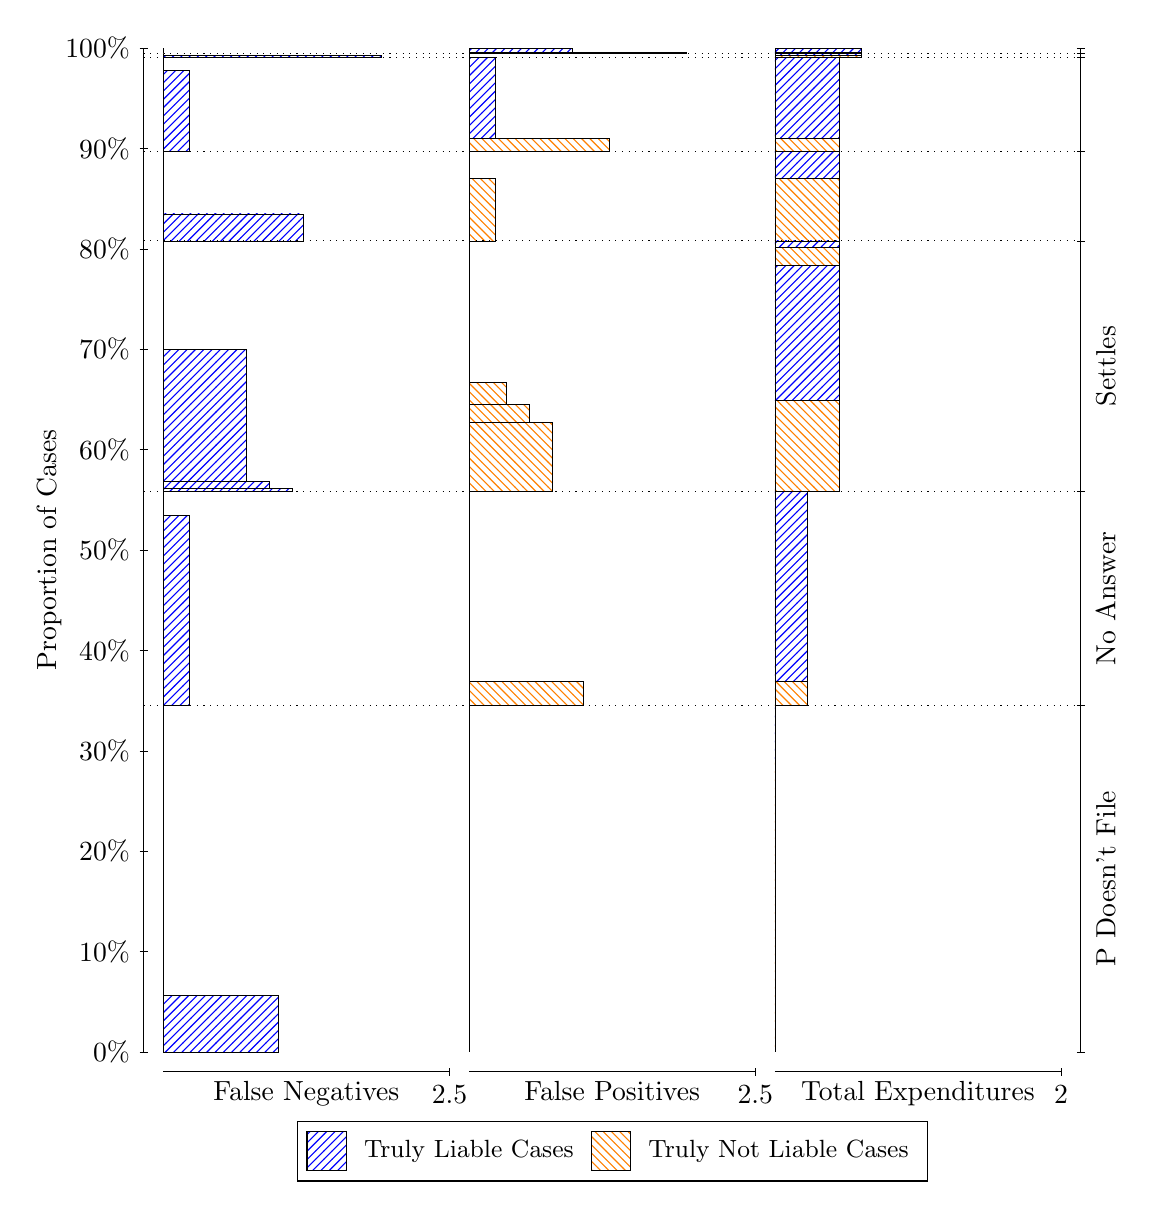
\begin{tikzpicture}
\draw[black, very thin] (1.5,1.75) -- (1.5,14.5);
\node[rotate=90, text=black, anchor=center] at (0.3, 8.125) {Proportion of Cases};
\draw[black, very thin] (1.45,1.75) -- (1.55,1.75);
\node[text=black, anchor=east] at (1.45, 1.75) {0\%};
\draw[black, very thin] (1.45,3.025) -- (1.55,3.025);
\node[text=black, anchor=east] at (1.45, 3.025) {10\%};
\draw[black, very thin] (1.45,4.3) -- (1.55,4.3);
\node[text=black, anchor=east] at (1.45, 4.3) {20\%};
\draw[black, very thin] (1.45,5.575) -- (1.55,5.575);
\node[text=black, anchor=east] at (1.45, 5.575) {30\%};
\draw[black, very thin] (1.45,6.85) -- (1.55,6.85);
\node[text=black, anchor=east] at (1.45, 6.85) {40\%};
\draw[black, very thin] (1.45,8.125) -- (1.55,8.125);
\node[text=black, anchor=east] at (1.45, 8.125) {50\%};
\draw[black, very thin] (1.45,9.4) -- (1.55,9.4);
\node[text=black, anchor=east] at (1.45, 9.4) {60\%};
\draw[black, very thin] (1.45,10.675) -- (1.55,10.675);
\node[text=black, anchor=east] at (1.45, 10.675) {70\%};
\draw[black, very thin] (1.45,11.95) -- (1.55,11.95);
\node[text=black, anchor=east] at (1.45, 11.95) {80\%};
\draw[black, very thin] (1.45,13.225) -- (1.55,13.225);
\node[text=black, anchor=east] at (1.45, 13.225) {90\%};
\draw[black, very thin] (1.45,14.5) -- (1.55,14.5);
\node[text=black, anchor=east] at (1.45, 14.5) {100\%};

\draw[black, very thin] (13.4,1.75) -- (13.4,14.5);
\draw[black, very thin] (13.35,1.75) -- (13.45,1.75);
\node[anchor=west] at (13.35, 1.75) {};
\draw[black, very thin] (13.35,6.1471) -- (13.45,6.1471);
\node[anchor=west] at (13.35, 6.1471) {};
\draw[black, very thin] (13.35,8.873) -- (13.45,8.873);
\node[anchor=west] at (13.35, 8.873) {};
\draw[black, very thin] (13.35,12.05) -- (13.45,12.05);
\node[anchor=west] at (13.35, 12.05) {};
\draw[black, very thin] (13.35,13.186) -- (13.45,13.186);
\node[anchor=west] at (13.35, 13.186) {};
\draw[black, very thin] (13.35,14.384) -- (13.45,14.384);
\node[anchor=west] at (13.35, 14.384) {};
\draw[black, very thin] (13.35,14.43) -- (13.45,14.43);
\node[anchor=west] at (13.35, 14.43) {};
\draw[black, very thin] (13.35,14.5) -- (13.45,14.5);
\node[anchor=west] at (13.35, 14.5) {};

\draw[black, very thin, pattern color=blue, pattern=north east lines] (1.75,1.75) rectangle (3.2033,2.4668);
\draw[black, very thin, pattern color=orange, pattern=north west lines] (1.75,2.4668) rectangle (1.75,6.1471);
\draw[black, very thin, pattern color=blue, pattern=north east lines] (1.75,6.1471) rectangle (2.077,8.5626);
\draw[black, very thin, pattern color=orange, pattern=north west lines] (1.75,8.5626) rectangle (1.75,8.873);
\draw[black, very thin, pattern color=blue, pattern=north east lines] (1.75,8.873) rectangle (3.385,8.9116);
\draw[black, very thin, pattern color=blue, pattern=north east lines] (1.75,8.9116) rectangle (3.0943,8.9965);
\draw[black, very thin, pattern color=blue, pattern=north east lines] (1.75,8.9965) rectangle (2.8037,10.673);
\draw[black, very thin, pattern color=orange, pattern=north west lines] (1.75,10.673) rectangle (1.75,12.05);
\draw[black, very thin, pattern color=blue, pattern=north east lines] (1.75,12.05) rectangle (3.5303,12.395);
\draw[black, very thin, pattern color=orange, pattern=north west lines] (1.75,12.395) rectangle (1.75,13.186);
\draw[black, very thin, pattern color=blue, pattern=north east lines] (1.75,13.186) rectangle (2.077,14.214);
\draw[black, very thin, pattern color=orange, pattern=north west lines] (1.75,14.214) rectangle (1.75,14.384);
\draw[black, very thin, pattern color=blue, pattern=north east lines] (1.75,14.384) rectangle (4.5113,14.404);
\draw[black, very thin, pattern color=orange, pattern=north west lines] (1.75,14.404) rectangle (1.75,14.43);
\draw[black, very thin, pattern color=orange, pattern=north west lines] (1.75,14.43) rectangle (1.75,14.449);
\draw[black, very thin, pattern color=blue, pattern=north east lines] (1.75,14.449) rectangle (1.75,14.5);
\draw[black, very thin, pattern color=orange, pattern=north west lines] (5.6333,1.75) rectangle (5.6333,5.4303);
\draw[black, very thin, pattern color=blue, pattern=north east lines] (5.6333,5.4303) rectangle (5.6333,6.1471);
\draw[black, very thin, pattern color=orange, pattern=north west lines] (5.6333,6.1471) rectangle (7.0867,6.4576);
\draw[black, very thin, pattern color=blue, pattern=north east lines] (5.6333,6.4576) rectangle (5.6333,8.873);
\draw[black, very thin, pattern color=orange, pattern=north west lines] (5.6333,8.873) rectangle (6.687,9.75);
\draw[black, very thin, pattern color=orange, pattern=north west lines] (5.6333,9.75) rectangle (6.3963,9.9729);
\draw[black, very thin, pattern color=orange, pattern=north west lines] (5.6333,9.9729) rectangle (6.1057,10.25);
\draw[black, very thin, pattern color=blue, pattern=north east lines] (5.6333,10.25) rectangle (5.6333,12.05);
\draw[black, very thin, pattern color=orange, pattern=north west lines] (5.6333,12.05) rectangle (5.9603,12.842);
\draw[black, very thin, pattern color=blue, pattern=north east lines] (5.6333,12.842) rectangle (5.6333,13.186);
\draw[black, very thin, pattern color=orange, pattern=north west lines] (5.6333,13.186) rectangle (7.4137,13.357);
\draw[black, very thin, pattern color=blue, pattern=north east lines] (5.6333,13.357) rectangle (5.9603,14.384);
\draw[black, very thin, pattern color=orange, pattern=north west lines] (5.6333,14.384) rectangle (5.6333,14.41);
\draw[black, very thin, pattern color=blue, pattern=north east lines] (5.6333,14.41) rectangle (5.6333,14.43);
\draw[black, very thin, pattern color=orange, pattern=north west lines] (5.6333,14.43) rectangle (8.3947,14.449);
\draw[black, very thin, pattern color=blue, pattern=north east lines] (5.6333,14.449) rectangle (6.9413,14.5);
\draw[black, very thin, pattern color=orange, pattern=north west lines] (9.5167,1.75) rectangle (9.5167,5.4303);
\draw[black, very thin, pattern color=blue, pattern=north east lines] (9.5167,5.4303) rectangle (9.5167,6.1471);
\draw[black, very thin, pattern color=orange, pattern=north west lines] (9.5167,6.1471) rectangle (9.9254,6.4576);
\draw[black, very thin, pattern color=blue, pattern=north east lines] (9.5167,6.4576) rectangle (9.9254,8.873);
\draw[black, very thin, pattern color=orange, pattern=north west lines] (9.5167,8.873) rectangle (10.334,10.027);
\draw[black, very thin, pattern color=blue, pattern=north east lines] (9.5167,10.027) rectangle (10.334,11.743);
\draw[black, very thin, pattern color=orange, pattern=north west lines] (9.5167,11.743) rectangle (10.334,11.966);
\draw[black, very thin, pattern color=blue, pattern=north east lines] (9.5167,11.966) rectangle (10.334,12.05);
\draw[black, very thin, pattern color=orange, pattern=north west lines] (9.5167,12.05) rectangle (10.334,12.842);
\draw[black, very thin, pattern color=blue, pattern=north east lines] (9.5167,12.842) rectangle (10.334,13.186);
\draw[black, very thin, pattern color=orange, pattern=north west lines] (9.5167,13.186) rectangle (10.334,13.357);
\draw[black, very thin, pattern color=blue, pattern=north east lines] (9.5167,13.357) rectangle (10.334,14.384);
\draw[black, very thin, pattern color=orange, pattern=north west lines] (9.5167,14.384) rectangle (10.607,14.41);
\draw[black, very thin, pattern color=blue, pattern=north east lines] (9.5167,14.41) rectangle (10.607,14.43);
\draw[black, very thin, pattern color=orange, pattern=north west lines] (9.5167,14.43) rectangle (10.607,14.449);
\draw[black, very thin, pattern color=blue, pattern=north east lines] (9.5167,14.449) rectangle (10.607,14.5);
\draw[black, dotted] (1.5,6.1471) -- (13.4,6.1471);
\draw[black, dotted] (1.5,8.873) -- (13.4,8.873);
\draw[black, dotted] (1.5,12.05) -- (13.4,12.05);
\draw[black, dotted] (1.5,13.186) -- (13.4,13.186);
\draw[black, dotted] (1.5,14.384) -- (13.4,14.384);
\draw[black, dotted] (1.5,14.43) -- (13.4,14.43);
\draw[black, very thin] (1.75,1.5) -- (5.3833,1.5);
\node[text=black, anchor=north] at (3.5667, 1.5) {False Negatives};
\draw[black, very thin] (5.3833,1.45) -- (5.3833,1.55);
\node[text=black, anchor=north] at (5.3833, 1.45) {2.5};

\draw[black, very thin] (5.6333,1.5) -- (9.2667,1.5);
\node[text=black, anchor=north] at (7.45, 1.5) {False Positives};
\draw[black, very thin] (9.2667,1.45) -- (9.2667,1.55);
\node[text=black, anchor=north] at (9.2667, 1.45) {2.5};

\draw[black, very thin] (9.5167,1.5) -- (13.15,1.5);
\node[text=black, anchor=north] at (11.333, 1.5) {Total Expenditures};
\draw[black, very thin] (13.15,1.45) -- (13.15,1.55);
\node[text=black, anchor=north] at (13.15, 1.45) {2};

\node[text=black, centered, rotate=90] at (13.72, 3.9486) {P Doesn't File};
\node[text=black, centered, rotate=90] at (13.72, 7.5101) {No Answer};
\node[text=black, centered, rotate=90] at (13.72, 10.462) {Settles};





\draw (7.449999999999999,1.5) node[draw=none] (baseCoordinate) {};
\begin{scope}[align=center]
        \matrix[scale=0.5, draw=black, below=0.5cm of baseCoordinate, nodes={draw}, column sep=0.1cm]{
            \node[rectangle, draw, minimum width=0.5cm, minimum height=0.5cm, pattern color=blue, pattern=north east lines] {}; &
            \node[draw=none, font=\small, text=black] (B) {Truly Liable Cases}; &
            \node[rectangle, draw, minimum width=0.5cm, minimum height=0.5cm, pattern color=orange, pattern=north west lines] {}; &
            \node[draw=none, font=\small, text=black] (B) {Truly Not Liable Cases}; \\
            };
\end{scope}

\end{tikzpicture}
\end{document}